\documentclass[12pt]{article}
\usepackage{graphicx}
\usepackage{url}
\usepackage{float}
\graphicspath{ {./images/} }

\begin{document}
	
\begin{titlepage}
	\begin{center}
		\huge
		Artificial Intelligence In Healthcare\\
		\vspace{0.2cm}
		\normalsize
		A case study in rehabilitation
		
		\vspace{1.5cm}
		\large
		A report submitted in partiall fulfillment of the requirement for \\Seminar I(CS69101)\\
		
		\vspace{4.5cm}
		Under the guidance of\\
		Dr. Aritra Hazra
		
		\vfill

		\Large
		Ankit Kumar Verma\\
		\normalsize
		21CS60A04\\
		Master of Technology\\
		Department of Computer Science and Engineering\\
		Indian Institute of Technology Kharagpur\\
	\end{center}
\end{titlepage}

\tableofcontents
\newpage

\section{Introduction}
\paragraph{}
Artificial Intelligence (AI) is a simulation of human cognitive functions such as learning and problem-solving. It generally applies to computational technologies that emulate mechanisms assisted by human intelligence, such as thought, deep learning, adaptation, engagement, and sensory understanding.\cite{Silvana Secinaro} The various sub-fields of AI are centered around particular goals that include reasoning, knowledge representation, planning, learning, natural language processing, and perception.\cite{AI}

\paragraph{}
AI can gather and organize vast volumes of data in order to draw inferences and estimates that are outside of the human ability to comprehend manually. It also improves organizational efficiency while lowering the risk of a mistake, and it identifies unusual patterns, such as spam and frauds, instantaneously to alert organizations about suspicious behavior, among other things.\cite{Madhurjya Chowdhury}

\paragraph{}
Overall, there are two basic tasks that AI tries to achieve i.e. classification and prediction. For a human to differentiate between a cat’s image and a dog’s image, he/she learns different features of the species such as body shape, size, color, etc. Similarly, AI machines too when fed with a number of images of cats and dogs, can learn the features of the species and classify them.

\paragraph{}
The other important task that AI machines try to achieve is prediction. Like humans, who can analyze past data, events, and trends to predict a future event/outcome, AI machines too can establish patterns in data and predict a future outcome for a given input. Various implementations has been in place such as weather forecasting, stock market prediction, etc.

\paragraph{}
Today, AI is being used in different industries such as healthcare, automotive, finance, transportation, travel, eCommerce, etc. The possibilities for AI are endless. One can imagine the possibilities such as sending a car to pick up kids from school, using drones to deliver e-commerce products, asking robots to carry out household chores, etc. Another possibility that is being researched by MIT is creating AI robots with a biological brain made up of human neurons - “connecting a human brain with a computer network via an implant”.\cite{Kevin Warwick}

\newpage


\section{History and Rise of Artificial Intelligence}
\paragraph{}
The concept of machines being taught to perform tasks that require human thinking and reasoning dates back to antiquity. However, it wasn’t until the 1950s where the true possibility of Artificial Intelligence was explored. 

\paragraph{}
Computer Scientist, Alan Turing, suggested that if humans use available information, as well as reason, to solve problems and make decisions - then why can’t machines do the same thing? In 1950, he presented the idea of Artificial Intelligence and defined them as “thinking machines” in his paper - Computing Machinery and Intelligence. In his paper, Turing established that binary mathematics could be used to solve any conceivable problem.\cite{A. M. TURING} He also outlined the machines and how to test their intelligence. However, his idea did not advance as computers of that time could only execute commands and not store them.

\paragraph{}
In the 60s, computers flourished. They were faster, more affordable, and were able to store more information. It was during this time, early demonstration of AI could be seen. A chatbot named Eliza was created by MIT Artificial Intelligence Laboratory. In 1986, the first autonomous car was built by C.M.U with neural networks. The concept which was established in the 80s is finally coming to realization for the mass. Various tech giants from different parts of the world are working on autonomous cars to make them a reality in our daily life. 

\paragraph{}
The 80s saw an exponential increase in computing power. The volume of data generation exploded. It was during this time that AI techniques and statistical models were being looked at to move from academic and defense applications into the business world. This era showed that AI could be used to predict stock prices and that statistical modeling could be incredibly lucrative when applied to the right problem.

\paragraph{}
The field of AI is more than half a century old now. AI machines such as DeepBlue\cite{DeepBlue} and DeepMind\cite{DeepMind} have been built to an extent that they are able to beat humans at games such as Chess and AlphaGo respectively which were created by humans themselves.

\newpage

\section{AI in Healthcare}
\paragraph{}
AI has been involved in medicine since as early as the 1950s when physicians made the first attempts to improve their diagnoses using computer-aided programs. Today AI is being used in different domains of digital healthcare.\cite{Silvana Secinaro}\\

\begin{figure}[h]
	\begin{center}
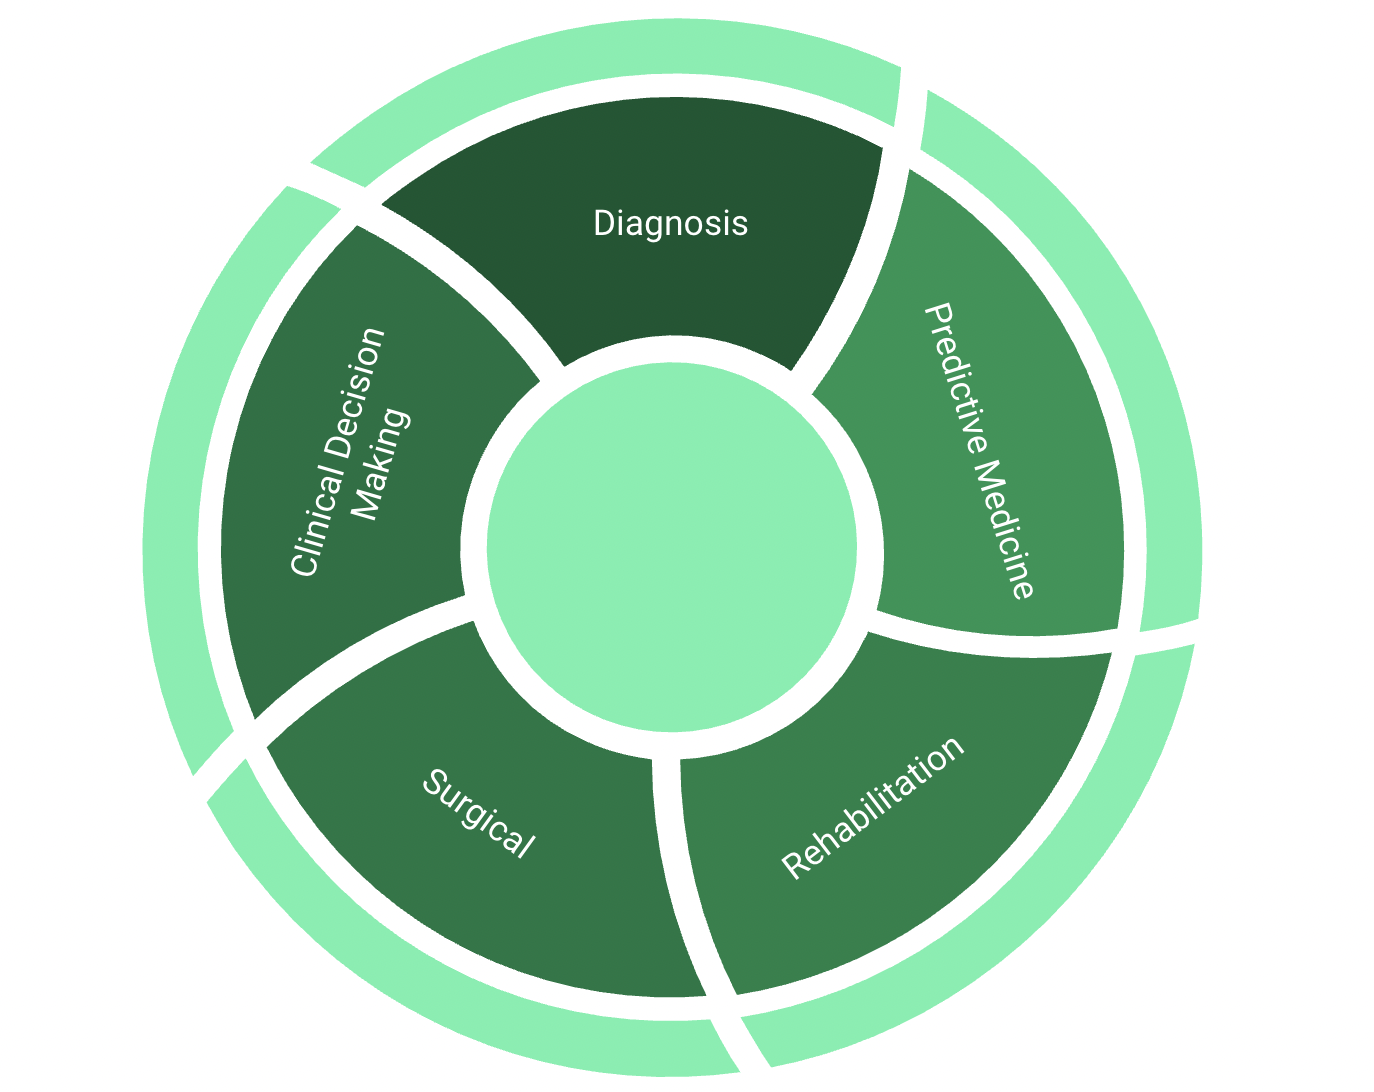
\includegraphics[height=10cm,width=13cm]{HealthSectors}
\end{center}
\caption{Different Domains of Healthcare}
\end{figure}


\paragraph{}
AI has been a disruptive innovation in healthcare. With its sophisticated algorithms and
several applications, AI has assisted doctors and medical professionals in the domains of health information systems, geocoding health data, epidemic and syndromic surveillance, predictive modelling and decision support, and medical imaging.

\paragraph{}
AI has the potential to support comprehensive health services management. The AI applications can support doctors, nurses, and administrators in their work by providing constant, possibly real-time medical information updates from various sources, including journals, textbooks, and clinical practices. 

\paragraph{}
Like any other sector, Healthcare is adopting AI technologies at a very rapid pace. We can already see the impact of AI technologies in different domains of healthcare such as diagnosis, predictive medicine, rehabilitation, surgical, and clinical decision-making. 

\paragraph{}
Predictive medicine is another area where AI applications are making a difference with disease prediction and diagnosis treatment, outcome prediction, and prognosis evaluation. It is estimated that an individual creates about 0.4 TB of medical data, 6 TB of genomic data, and 1,100 TB of environmental and daily life data throughout a lifetime. Earlier, the technology was not advanced enough to handle this kind of volume. \cite{Jeong Hyeon Han}

\paragraph{}
However, AI technologies today can ingest, analyze, and report large volumes of data also referred to as medical big data. AI can identify meaningful relationships in raw data and thus can support diagnostic, treatment, and prediction outcomes in many medical situations. AI can also deal with the vast amount of data produced in medicine and find new information that would otherwise remain hidden in the mass of medical big data. \cite{Silvana Secinaro}

\paragraph{}
These technologies can help design and develop new drugs, monitor patients, and personalise patient treatment plans. Additionally, AI can contribute to optimizing logistics processes, for instance, realizing drugs and equipment in a just-in-time supply system based totally on predictive algorithms.


\paragraph{}
Recently, robotic-assisted surgery has gained acceptance in different medical fields, such as urological, colorectal, cardiothoracic, orthopedic, maxillofacial, and neurosurgery applications.\cite{Silvana Secinaro}

\newpage

\section{AI in Rehabilitation}
\paragraph{}
A person suffers from paralysis or paresis because of a number of reasons. The neurological condition could be caused due to an accident, spinal cord injury, stroke, etc. In this condition, the patient loses one or more locomotive motions. \\

\begin{figure}[h]
	\begin{center}
		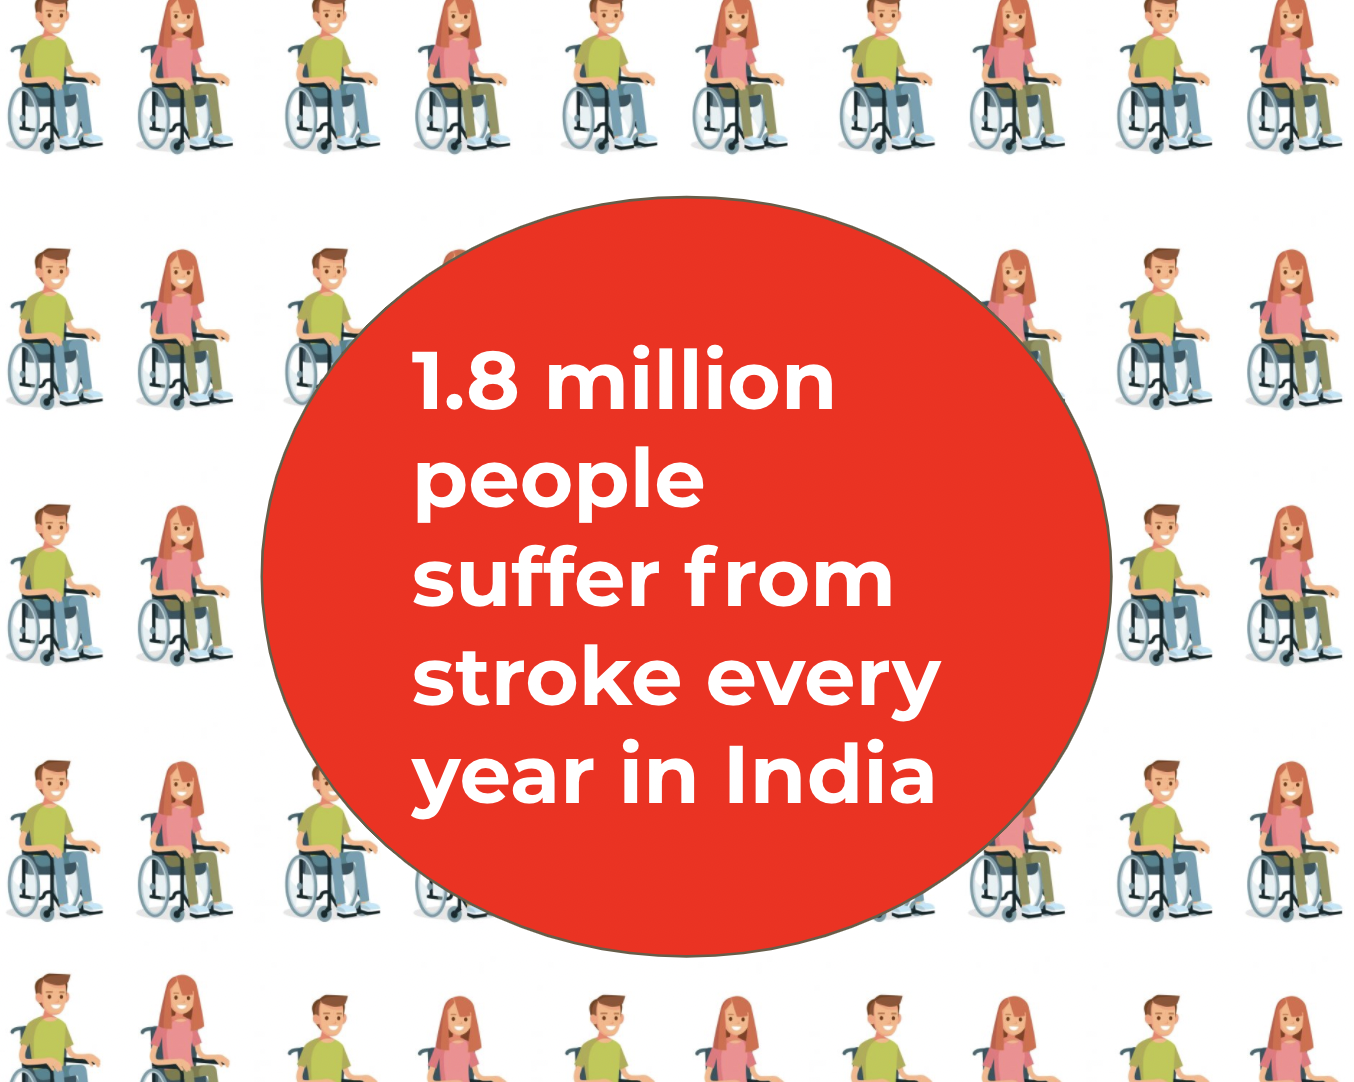
\includegraphics[height=8cm,width=10cm]{StrokeStatistics}
	\end{center}
	\caption{Stroke Statistics}
\end{figure}

\paragraph{}
According to the Stroke Association of India, about 1.8 million people suffer from stroke every year. And these numbers are rising every year. The world statistics are also on the same trend. The number of patients suffering from a neurological condition that requires rehabilitation care is on an increasing trend while the demand for healthcare professionals required in this domain is in shortage.

\paragraph{}
The patients suffering from these neurological conditions have to undergo rehabilitation for a long duration which may last for months or years. During the recovery period, patients perform various repetitive tasks based on the condition.

\paragraph{}
There is room for various technologies to pitch in this domain to make the recovery process more efficient in terms of human assistance. One such example is the usage of robots which can help the patients during the treatment.

\paragraph{}
Many robots have been created to assist a number of neurological conditions. These robots when clubbed with artificial intelligence technologies can make the recovery process a lot efficient and faster. One such example of such a robot in the industry is Hope of Hand. These robots can predict the intent of the patient and thus help the patient to carry out the activities.

\begin{figure}[h]
	\begin{center}
		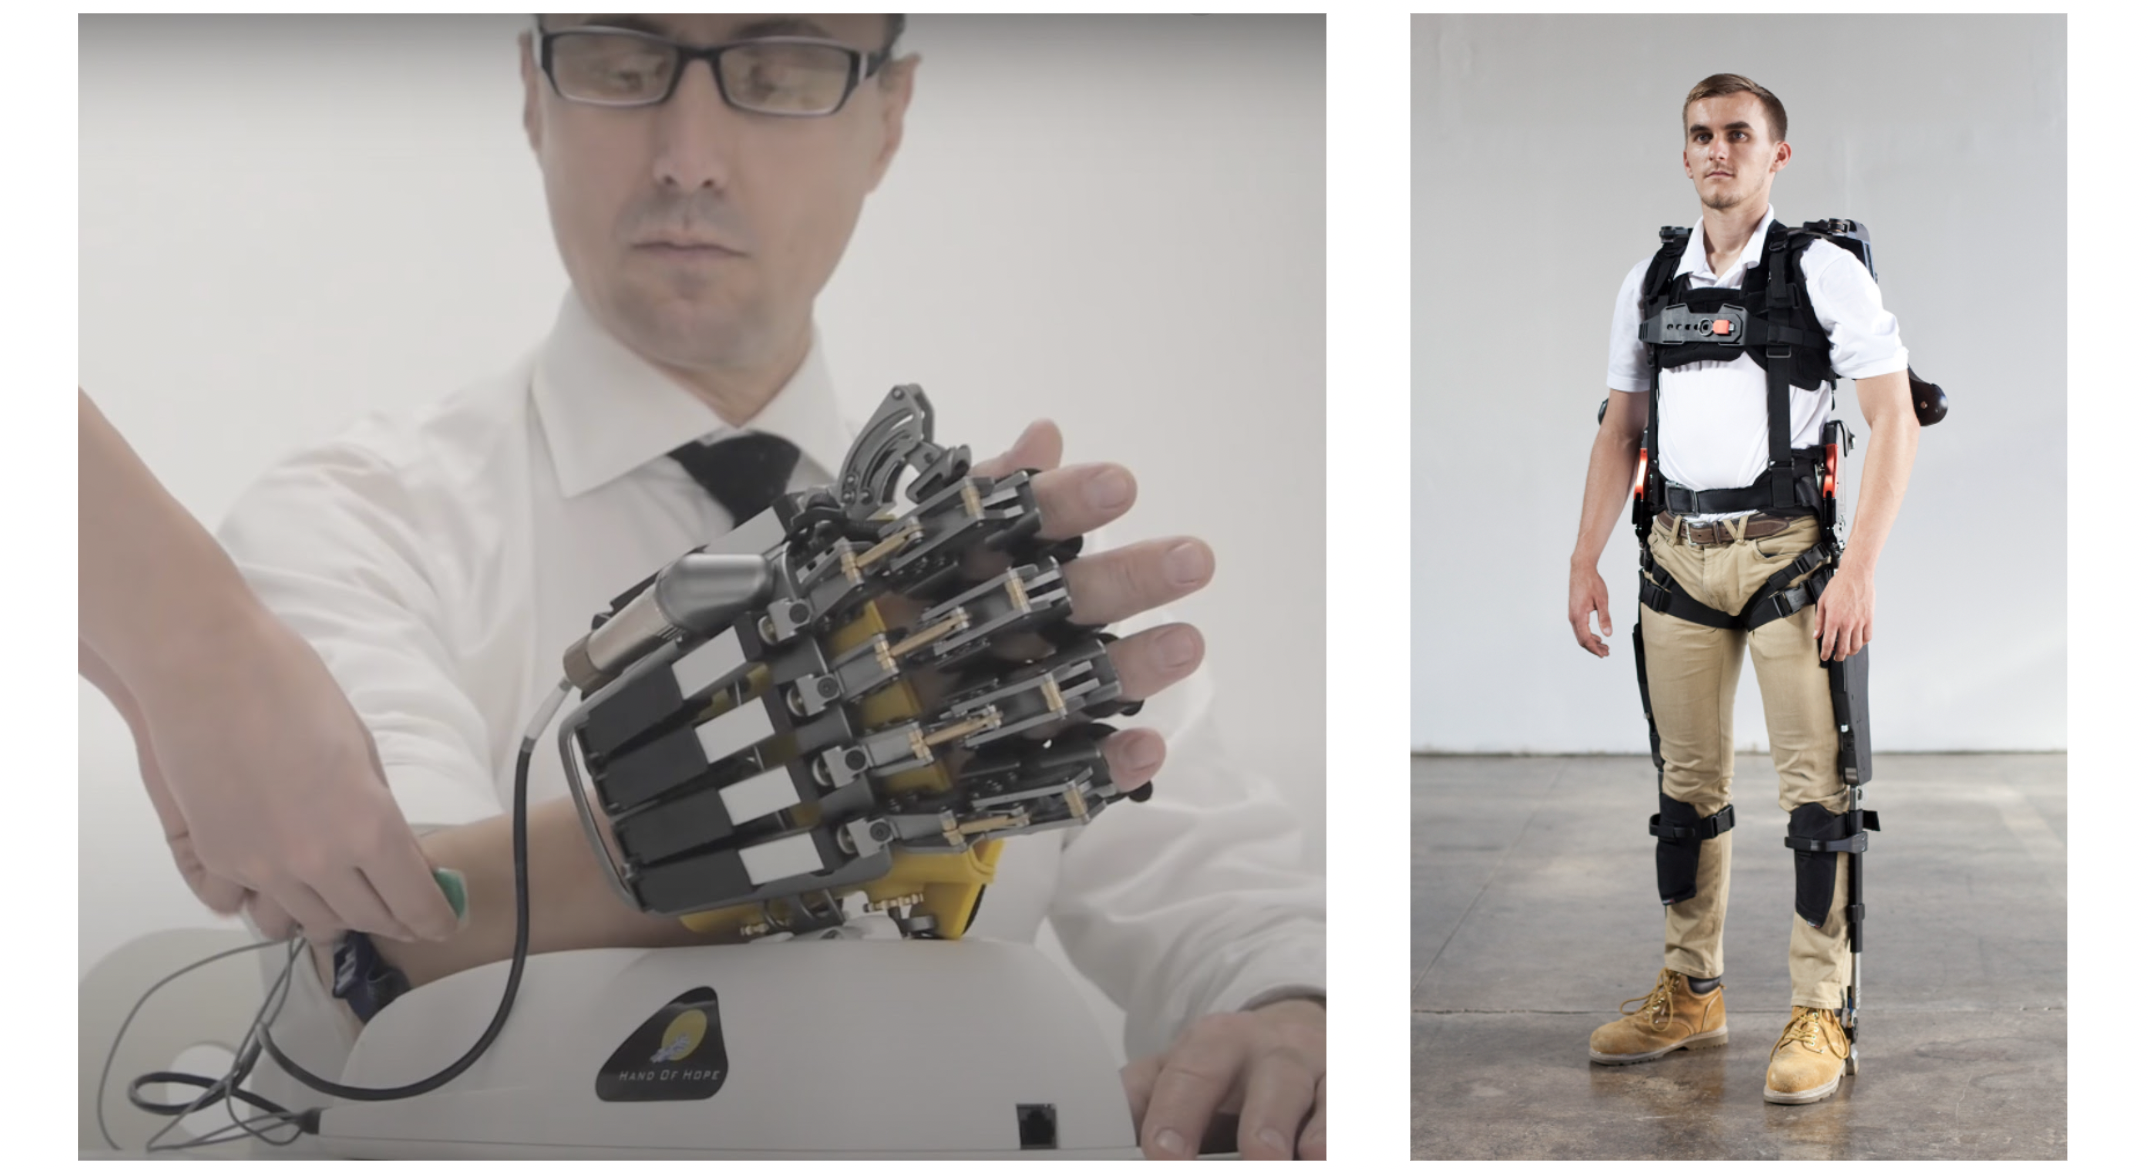
\includegraphics[height=8cm,width=15cm]{Patients}
	\end{center}
	\caption{Patients with neurologial condition}
\end{figure}

\paragraph{}
The above two pictures are of patients suffering from different neurological conditions and are going through rehabilitation. In the picture on left, the patient is wearing a robot named “Hope of Hand”. This robot helps the patient to open and close his finger when he intents. In the right image, the patient is wearing an exoskeleton, here the robot helps the patient move. In all these robots, one of the fundamental challenges is to predict the locomotion mode based upon the intent of the patient. Various literature has been published on the same. One of the highly cited ones is “SVM classification of locomotion modes using surface electromyography for applications in rehabilitation robotics”.\cite{E. Ceseracciu}  

\newpage

\subsection{Classification of locomotion modes using sEMG In Rehabilitation
	Robotics}

\paragraph{}
E. Ceseracciu, M. Reggiani, Z. Sawacha, M. Sartori, F. Spolaor, C. Cobelli, and E. Pagello tried to solve this problem by using Support Vector Machines with RBF kernel. Their paper “SVM classification of locomotion modes using surface electromyography for applications in rehabilitation robotics” provides a detailed experimental setup and discusses the results. \cite{E. Ceseracciu}


\subsubsection{Experimental Setup}

\paragraph{}
Three healthy subjects were recruited for the study, 2 female and 1 male, with a mean age of $29 \frac{+}{-} 8.9$ years and a mean body mass index (BMI) of $21.9 \frac{+}{-} 0.2 \frac{kg}{m^2}$.\\

\begin{figure}[h]
	\begin{center}
		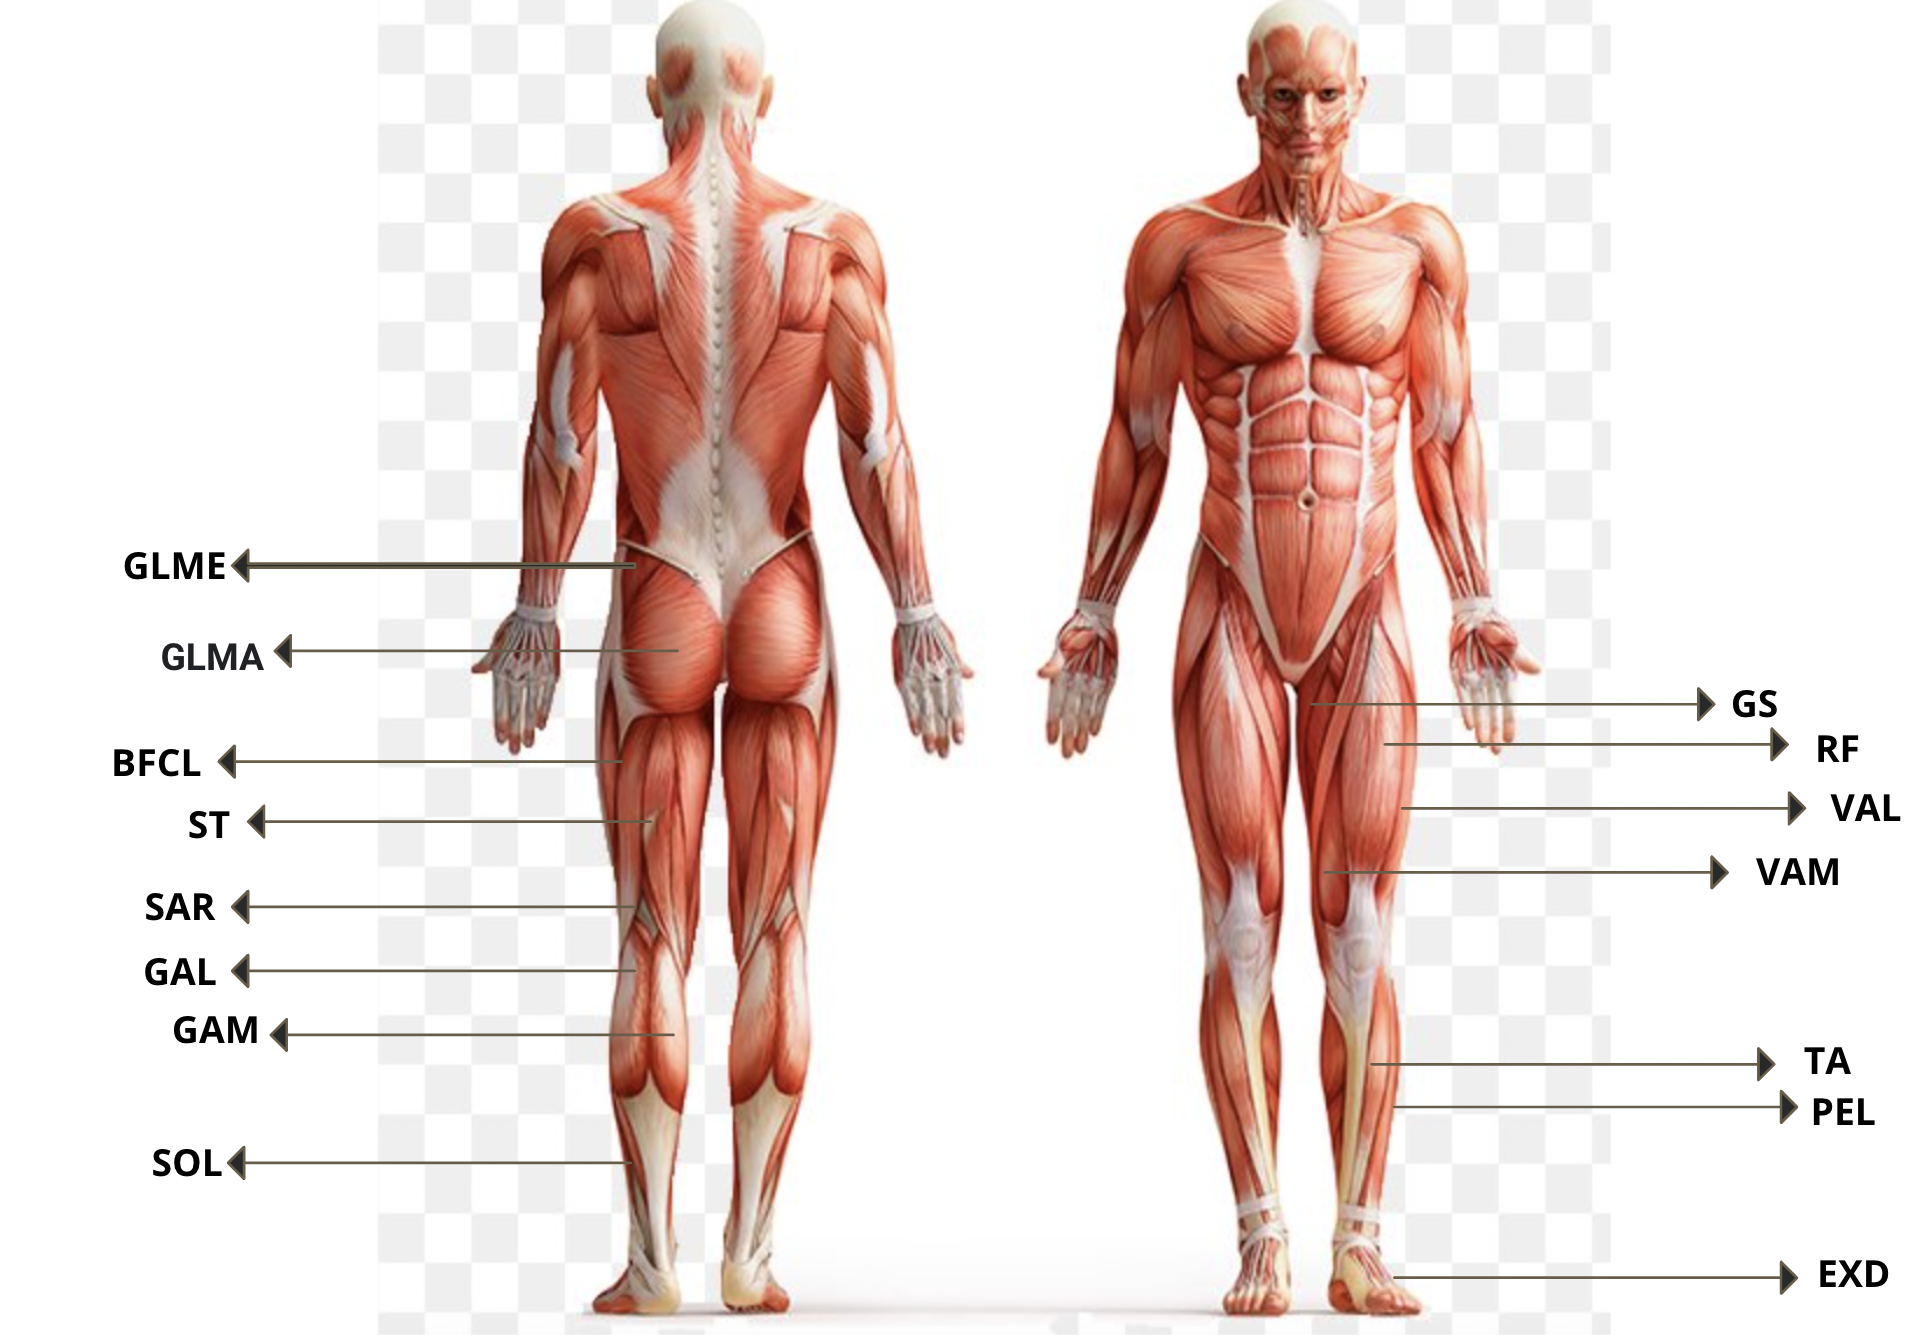
\includegraphics[height=8cm,width=13cm]{HumanBodyWithMarkedMuscles}
	\end{center}
	\caption{Human Body marked with muscles for monitoring}
\end{figure}

\paragraph{}
Each subject’s right leg muscular activity was monitored through a sixteen channels surface electromyography (sEMG) system (Pocket EMG, BTS Spa, frequency 1KHz). sEMG signals were detected from the following muscles:
\begin{enumerate}
	\item Gluteus Maximus (GLMA)
	\item Gluteus Medius (GLME)
	\item Sartorius (SAR)
	\item Rectus Femoris (RF) 
	\item Vastus Lateralis (VAL)
	\item Vastus Medialis (VAM)
	\item Gracilis (GR)
	\item Biceps Femoris Caput Longus (BFCL)
	\item Semitendinosus (ST)
	\item Tibialis Anterior (TA)
	\item Peroneus Longus (PEL)
	\item Gastrocnemius Lateral Head (GAL)
	\item Gastrocnemius Medial Head (GAM)
	\item Soleus (SOL) 
	\item Extensor Digitorum Brevis (EXD)
\end{enumerate}

\paragraph{}
After the attachment of the foot switches, subjects were allowed to walk until they were comfortable on a surface covered by linoleum. They walked barefoot at self-selected pace in the gait lab 8m long and 3m wide. 

\paragraph{}
Each subject performed the following motion modes: Level Walking, Stepping Over an Obstacle, Turning Right, Ascending Stairs, Descending Stairs, Standing Still. 

\paragraph{}
During the static acquisition, subjects were asked to stand for $60 seconds$ in an upright position, with their feet $30^{\circ}$ apart and their arms along the body, and to look at a small achromatic circular target placed about $1 meter$ from the eyes.

\paragraph{}
Stepping over an obstacle was performed asking the subject to step over a wooden block of $14.5 cm$ height, $40 cm$ width and $28.5 cm$ depth, while walking.

\subsubsection{Signal Analysis}
\paragraph{}
With the experimental setup described above features were extracted from filtered EMG signals. The first and the last strides were excluded from each trial due to walking initiation and termination. Each subject’s gait speed was checked by means of the foot switches data in order to verify whether it fell within the normal range, since muscle activation is related to gait velocity. Timings of footContact and footOff events were identified by means of basographic and motion analysis data.

\begin{figure}[h]
	\begin{center}
		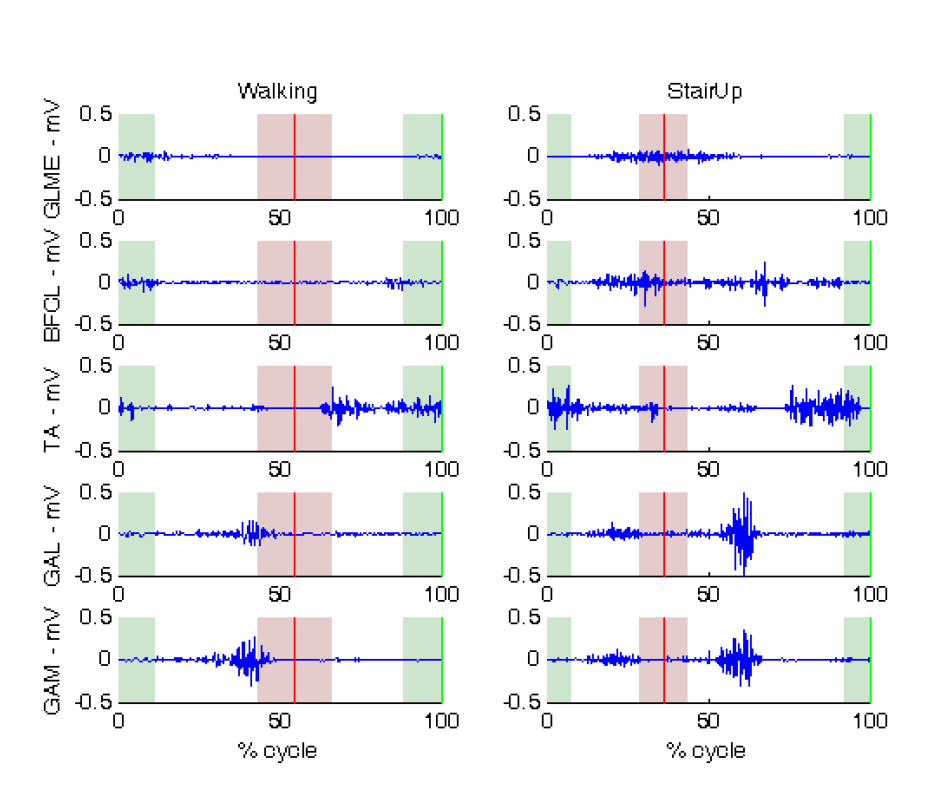
\includegraphics[height=8cm,width=12cm]{Signals}
	\end{center}
	\caption{FootContact and FootOff events are shown in green and red vertical lines respectively.}
\end{figure}

\paragraph{}
FootContact is characterized by the activation of any of the three foot switch signals; similarly, footOff is recognized by the deactivation of all signals.

\paragraph{}
In every analysis window, in order to provide a concise characterization suitable for classification both time-domain values, i.e. mean absolute value (MAV),
number of zero-crossings (ZC), waveform length (WFL), number of slope sign changes (SSC), root mean square (RMS) , and 3rd-order auto-regression coefficients (AR1,
AR2, AR3) were considered.

\paragraph{Mean Absolute Value (MAV)}\cite{Dennis Tkach}\\
This feature is the mean absolute value of signal $x$ in an analysis time window with $N$ samples. $x_k$ is the $k^{th}$ sample in this analysis window.\\\\
\begin{center}
$mAV = \frac{1}{N} \sum_{N}^{k=1}| x_k |$
\end{center}

\paragraph{Zero-crossings (ZC)}\cite{Dennis Tkach}\\
ZC is the number of times signal $x$ crosses zero within an analysis window; it is a simple measure associated with the frequency of the signal. To avoid signal crossing counts due to low-level noise, a threshold $\epsilon$ was included. The ZC count increased by one if\\
\begin{center}
$\{x_k > 0 \hspace{0.2cm} and \hspace{0.2cm} x_{k+1} < 0\}$ 
$\{x_k < 0 \hspace{0.2cm} and \hspace{0.2cm} x_{k+1} > 0\}$\\
and $|x_k - x_{k+1}| \geq \epsilon$
\end{center}

\paragraph{Waveform Length (WFL)}\cite{Dennis Tkach}\\
This feature provides a measure of the complexity of the signal. It is defined as the cumulative length of the EMG signal within the analysis window
\begin{center}
$wavLen=\sum_{N}^{k=1}|\Delta x_k|;where \Delta x_k = x_k - x_{k-1}$
\end{center}

\paragraph{Slope Sign Changes (SSC)}\cite{Dennis Tkach}\\
Slope sign change is related to signal frequency and is defined as the number of times that the slope of the EMG waveform changes sign within an analysis window. 
\begin{center}
$\{x_k > x_{k-1} \hspace{0.2cm} and \hspace{0.2cm} x_k > x_{k+1}\}\hspace{0.2cm} or \hspace{0.2cm}\{x_k < x_{k-1} \hspace{0.2cm} and \hspace{0.2cm} x_k < x_{k+1}\}$ \\
and $|x_k - x_{k-1}| \geq \epsilon \hspace{0.2cm} or \hspace{0.2cm} |x_k - x_{k+1}| \geq \epsilon$
\end{center}

\paragraph{Auto-Regression Coefficients(AR)}\cite{Dennis Tkach}\\
This feature models individual EMG signals as a linear autoregressive time series and provides information about the muscle's contraction state.\\
\begin{center}
$x_k = \sum_{i=1}^{p}a_i x_{k-1} + e_k$\\
\end{center}
where,\\ 
$a_i$ represents autoregressive coefficients, \\
$p$ is the AR model order, and \\
$e_k$ is the residual white noise\\

\subsubsection{SVM}
\paragraph{}
Support vector machine (SVM) algorithm is a well established technique to learn how to classify new data starting from a collection of classified events. With the features extracted from the signal analysis part, Support Vector Machine was used to classify the locomotion modes in the experiment. 

\paragraph{}
For the given experiment, libSVM\cite{libSVM}, a freely available implementation of the SVM
classifier was used. The whole set of experimental results has been obtained using the RBF kernel function.

\begin{center}
	$e^{\gamma}(a-b)^2$\\
\end{center}
Here, $\gamma$ is estimated by cross validation.\\
$a,b$ are data points.\\\\
Example:\\\\
$\gamma = 1, a = 2.5, b= 4$\\
$e = 0.11$\\\\
$\gamma = 1, a = 2, b = 16$\\
$e = \approx 0$ (for farther data points, $e$ is close to $0$)

\paragraph{}
While other kernels are available, authors have not compared their performances, as this was not part of the objectives of this work. Instead, authors have chosen a kernel that has already demonstrated good accuracy in the classification of upper limb motions. Additionally, the RBF kernel is usually a reasonable first choice as it can handle the nonlinear relation between class labels and attributes.\\

Some other areas where SVM has been successfully used in healthcare are:
\begin{itemize}
	\item SVM based on Sigmoid Kernel Function was used as a classifier to discriminate suspected patient data in cancer patient and normal subject classes. \cite{Liang Kou}
	\item SVM was used as a classifier to diagnose ovarian cancer based on amino acids. \cite{Farid A. Badria}
	\item Detection of outliers with one-class SVM in healthcare datasets.\cite{Roy Thomas}
\end{itemize}


\subsubsection{Validation}

\paragraph{}
Validation of the model was done with the help of LOOCV i.e Leave One Out Cross Validation. It is a special case of k-fold validation. The visual illustration of LOOCV is as below:

\begin{figure}[H]
	\begin{center}
		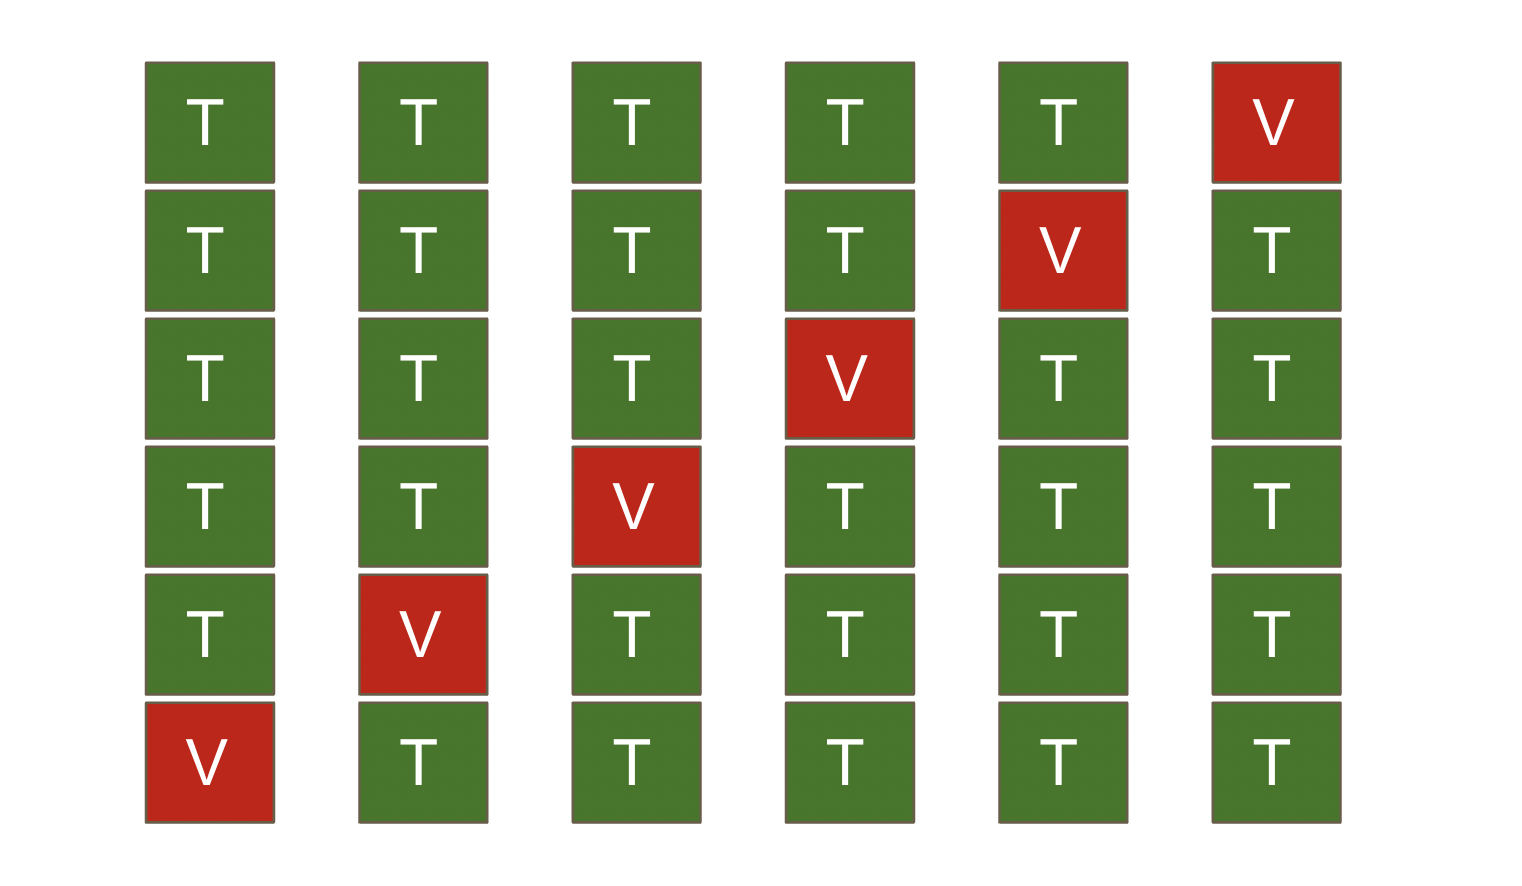
\includegraphics[height=6cm,width=11cm]{LOOCV}
	\end{center}
	\caption{LOOCV: Leave One Out Cross-Validation}
\end{figure}

\paragraph{}
This technique of validation is used when dataset is not very large. It gives reliable and unbiased estimate of model performance. This technique is easy to use and configure however it is computationally very costly.


\subsubsection{Results}
\paragraph{}
Classification accuracy for data samples composed of different subsets of EMG features from all muscles were analyzed. Best-case average accuracy (time-domain features, all muscles) ranged from $90\%$ (postContact) to $95\%$ (postOff).

\begin{figure}[h]
	\begin{center}
		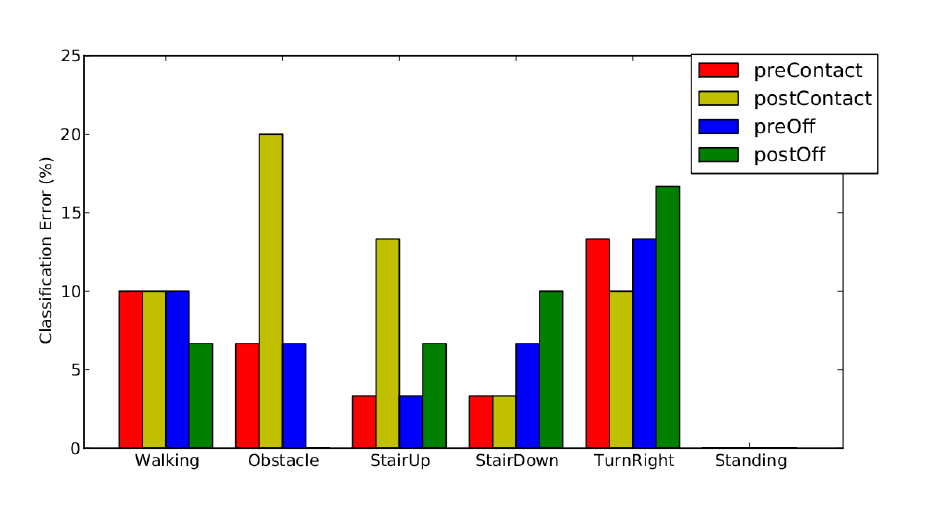
\includegraphics[height=8cm,width=15cm]{Error}
	\end{center}
	\caption{Average classification errors for each locomotion mode in the four phases.}
\end{figure}

\paragraph{}
In the above figure, it is evident that accuracy is phase dependant and locomotion modes are affected differently. Standing data is never misclassified.

\paragraph{}
Since the number and position of electrodes to be placed on a subject strongly affects the design of the exoskeleton and its usability, particular effort was made to reduce
the set of muscles that were needed to achieve acceptable classification results. Classification accuracy was therefore estimated on data samples obtained excluding one or more muscles from the feature extraction process. Some of the muscles have same biomechanic functions as others, example vasti (VAL and VAM) have the same role as knee extensors as RF, which also acts as hip flexor; glutei (GLMA and GLME) are both hip extensors; gastrocnemii (GAL and GAM) are knee flexors and are involved in plantarflexion of the foot, as well as soleus (SOL).

\paragraph{}
The below accuracy graph was obtained for the minimal set of muscles.

\begin{figure}[H]
	\begin{center}
		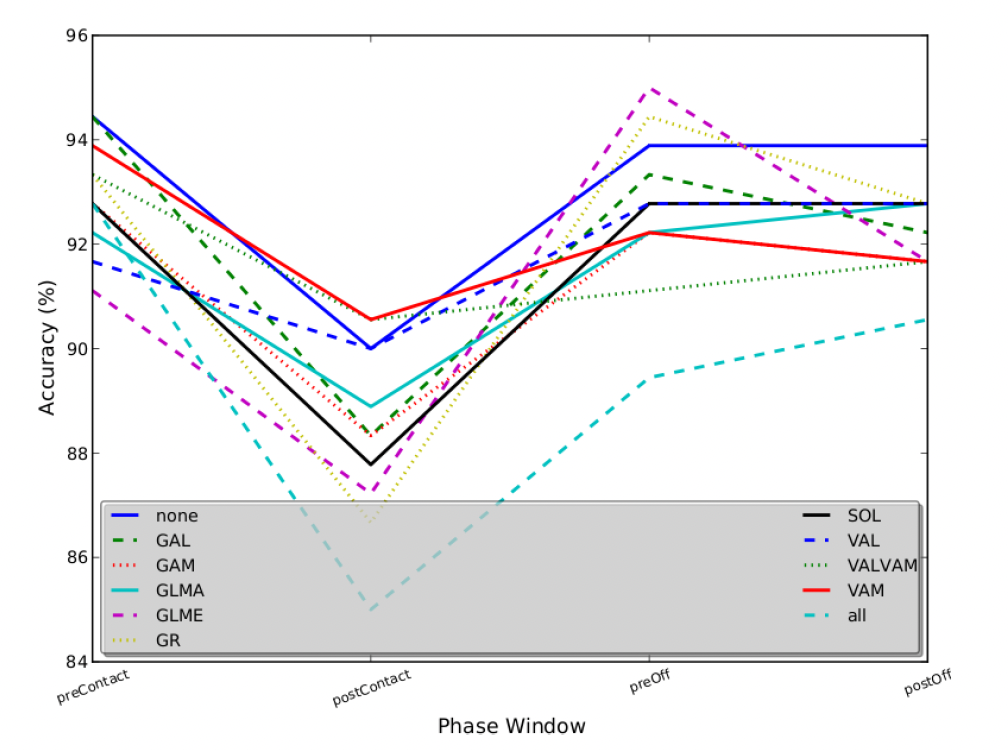
\includegraphics[height=8cm,width=14cm]{AccuracyReducedMuscles}
	\end{center}
	\caption{SVM classification accuracy for reduced sets of muscles, and optimal set of feature types.}
\end{figure}


\paragraph{}
When comparing the above results with the result obtained from all sets of muscles,
SVM was able to detect quite precisely the different motion modes.\\ The same is evident from the confusion matrix below.


\begin{figure}[H]
	\begin{center}
		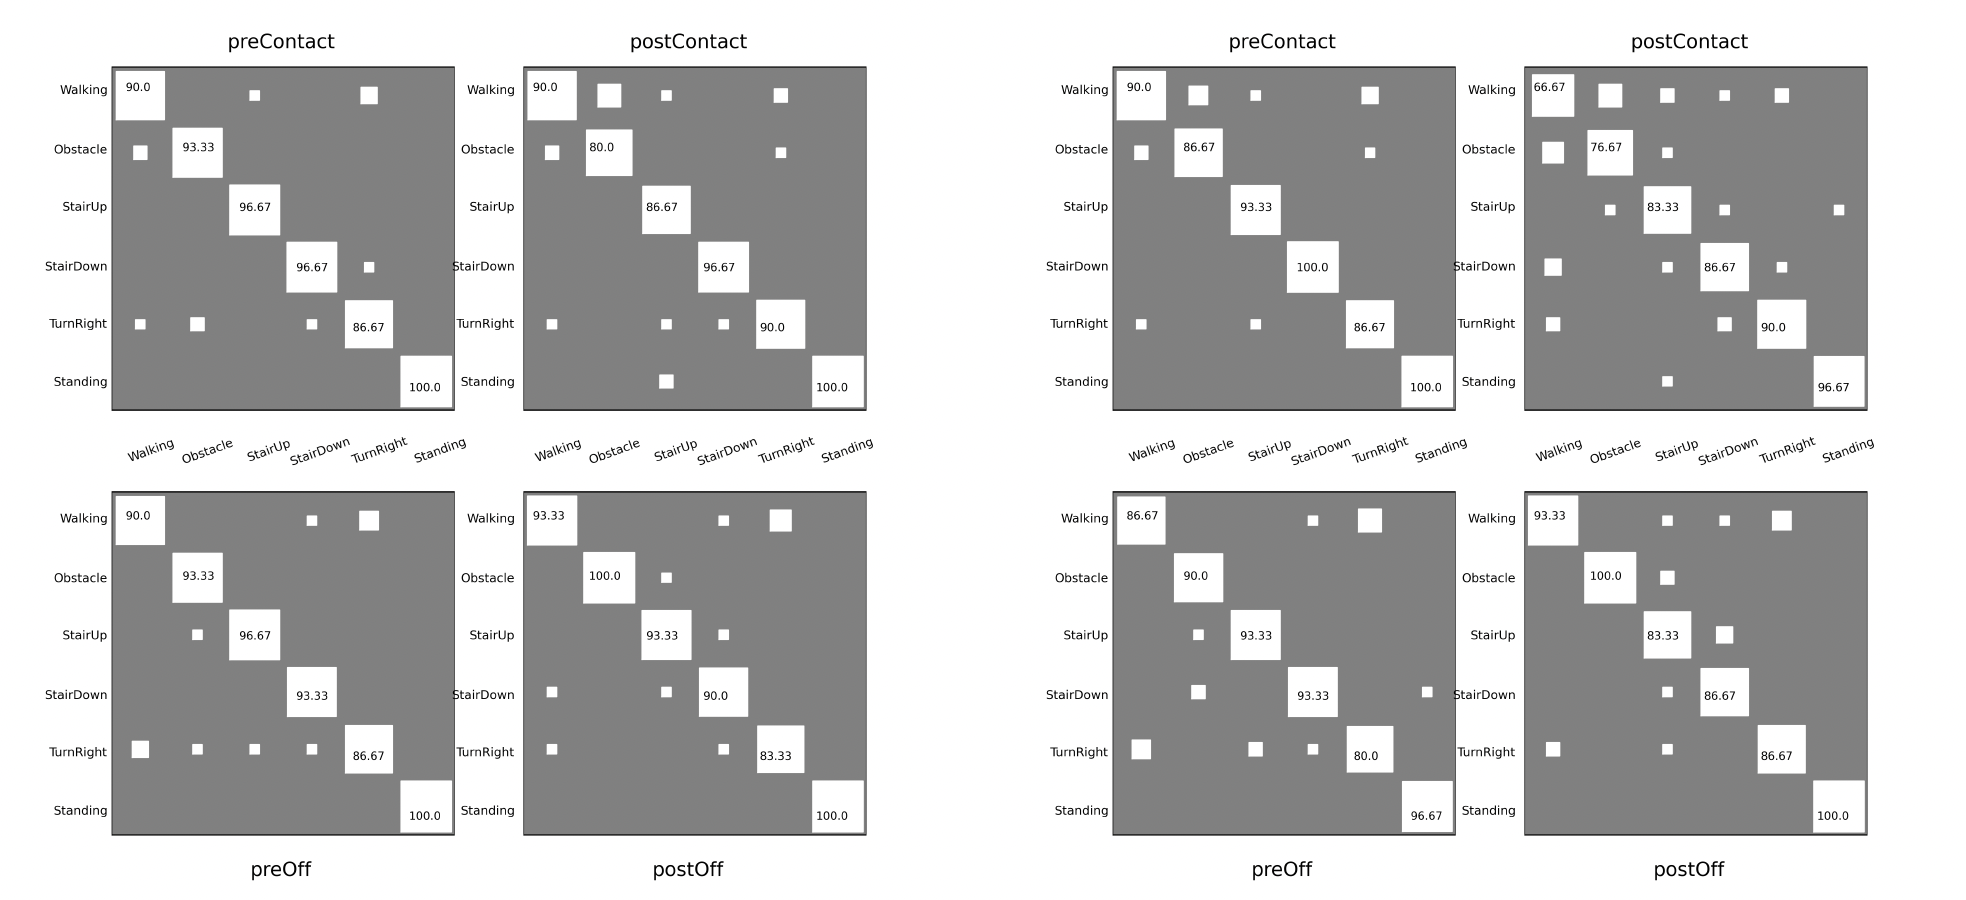
\includegraphics[height=7cm,width=15cm]{ConfusionMatrix}
	\end{center}
	\caption{SVM classification accuracy for reduced sets of muscles, and optimal set of feature types.}
\end{figure}

\subsubsection{Limitation of the approach}
\paragraph{}
External sensors such as wearable inertial measurement units (IMUs), optical distance sensors, and surface electromyography (sEMG) electrodes vary significantly with physiological factors including perspiration level, skin temperature, and subcutaneous fat thickness and thus predictions based on these inputs is not very accurate. Thus, for every experiment the results may be different. 

\subsubsection{Advanced Approaches}
\paragraph{}
Some advanced approaches have been tried out to overcome the limitations stated above. One of them is Translational Motion Tracking of Leg Joints for Enhanced Prediction of Walking Tasks. It aims to produce physiologically relevant signals without relying on a non-physiological and mechanically integrated sensor. It was been used in various bionics that are developed by the MIT researchers at Biomechatronics.

\paragraph{}
The author’s employed signals from an IMU(Inertial Measurement Unit) to generate physiologically meaningful estimates of leg joint translational motion and perform pattern recognition on the resulting signals to determine the target task of every stride. The performance of this novel approach is substantially more for walking prediction tasks then the previous methods. This method can be combined with other integrated sensing
modalities as part of a real-time task-adaptive leg prosthesis controller that is robust across users and physiological conditions. \cite{Roman Stolyarov}

\newpage 

\begin{thebibliography}{10}
\bibitem{E. Ceseracciu} E. Ceseracciu, M. Reggiani, Z. Sawacha, M. Sartori, F. Spolaor, C. Cobelli, E. Pagello, ``SVM classification of locomotion modes using surface electromyography
for applications in rehabilitation robotics," \emph{19th IEEE International Symposium on Robot and
Human Interactive Communication}, Sept 2010.

\bibitem{Roman Stolyarov} Roman Stolyarov, Gary Burnett, Hugh Herr, ``Translational Motion Tracking of Leg Joints for
Enhanced Prediction of Walking Tasks," \emph{IEEE Transactions on Biomedical Engineering}, vol. 65, pp 1-2, April 2018.

\bibitem{Silvana Secinaro} Silvana Secinaro, Davide Calandra, Aurelio Secinaro, Vivek Muthurangu, Paolo Biancone ``The role of artificial intelligence
in healthcare: a structured literature review," \emph{BMC Medical Informatics and Decision Making}, Apr 2021.

\bibitem{Jeong Hyeon Han} Jeong Hyeon Han, Joo Yeoun Lee, ``Digital Healthcare Industry and Technology Trends," \emph{2021 IEEE International Conference on Big Data and Smart Computing (BigComp)}, Jan 2021.

\bibitem{Liang Kou} Liang Kou, Ye Yuan, Jianguo Sun, Yun Lin, ``Prediction of Cancer Based on Mobile Cloud Computing and SVM," \emph{ 2017 International Conference on Dependable Systems and Their Applications (DSA)}, Nov 2017.

\bibitem{Farid A. Badria} Farid A. Badria, Nora Shoaip Mohammed Elmogy, A. M. Riad, Hosam Zaghloul, ``A Framework for Ovarian Cancer Diagnosis Based on Amino Acids Using Fuzzy-Rough Sets with SVM," \emph{The 2nd International Conference on Advanced Machine Learning Technologies and Applications (AMLT2014)}, Nov 2014.

\bibitem{Roy Thomas} Roy Thomas, J.E. Judith, ``Hybrid Outlier Detection in Healthcare Datasets
using DNN and One Class-SVM," \emph{2020 4th International Conference on Electronics, Communication and Aerospace Technology (ICECA)}, Nov 2020.

\bibitem{Dennis Tkach} Dennis Tkach, He Huang, Todd A Kuiken, ``Study of stability of time-domain features for electromyographic pattern recognition," \emph{Journal of NeuroEngineering and Rehabilitation}, May 2010.

\bibitem{AI} \emph{Wikipedia, free Encyclopedia}, \url{https://en.wikipedia.org/wiki/Artificial_intelligence}

\bibitem{DeepBlue} \emph{Wikipedia, free Encyclopedia}, \url{https://en.wikipedia.org/wiki/Deep_Blue_(chess_computer)}

\bibitem{DeepMind} \emph{Wikipedia, free Encyclopedia}, \url{https://en.wikipedia.org/wiki/DeepMind}

\bibitem{libSVM} C.-C. Chang and C.-J. Lin, \emph{LIBSVM: a library for
support vector machines}, \url{http://www.csie.ntu.edu.tw/ cjlin/libsvm.}

\bibitem{Madhurjya Chowdhury} Madhurjya Chowdhury,``The Evolution of Artificial Intelligence: Past, Present \& Future," \emph{Analytics Insight}, Aug 2021.

\bibitem{Kevin Warwick} Kevin Warwick,``The Future of Artificial Intelligence and Cybernetics," \emph{Technology Review}, Nov 2016.

\bibitem{A. M. TURING} A. M. TURING,``Computing Machinery And Intelligence," \emph{Mind, Volume LIX, Issue 236}, Oct 1950.

\end{thebibliography}

\end{document}
